\begin{frame}[fragile]{Why Finite Automata Are Not Enough}

    \begin{itemize}
        \item $L=\{a^{n}b^{n} \mid n \geq 1\}$ cannot be described by a FA.
        \item For a rejected word like \texttt{aaaabb},
        standard parsers identify the error at the end.
        %\item Standard parsers fail at the end of the input, obscuring the actual root cause (the extra bracket):
    \end{itemize}
    
    \vspace{0.4cm}

    \begin{columns}[T] % The [T] aligns the columns at the top
        
        % Left Column: C Code
        \begin{column}{0.46\textwidth}
            \textbf{Source Code:}
\begin{lstlisting}[language=C, basicstyle=\ttfamily\scriptsize, frame=single]
int main(){
    for(int i=0; i<10; i++){{ // Error
        printf("hello");
    }
}
\end{lstlisting}
        \end{column}

        % Right Column: Compiler Error
        \begin{column}{0.52\textwidth}
            \textbf{Parser Output:}
            % Note: Keep the verbatim text flush left so it doesn't add weird spaces
\begin{small}
\begin{verbatim}
error: expected '}' at end of input
5 | }
  | ^
\end{verbatim}
\end{small}
        \end{column}

    \end{columns}

\end{frame}

\section{Current Research: Explaining CFGs}

% \begin{frame}{Explaining Context-Free Grammars}
%     \begin{itemize}
%         \item Transition to Context-Free Grammars (CFGs).
%         \item Consider $G=(\{B, L, R\}, \{\texttt{(},\texttt{)}\}, R, B)$ for balanced parentheses, with rules $R$:
%     \end{itemize}
%     %
%     \begin{equation}
%     \begin{aligned}
%         B &\to \textbf{L} \, B \, \textbf{R} \, B & \text{(Rule 1)}\\
%         B &\to \textbf{L} \, B \, \textbf{R} & \text{(Rule 2)}\\
%         B &\to \textbf{L} \, \textbf{R} \, B & \text{(Rule 3)}\\
%         B &\to \textbf{L} \, \textbf{R} & \text{(Rule 4)}\\
%         \textbf{L} &\to \texttt{(} & \text{(Unary Rule 1)}\\
%         \textbf{R} &\to \texttt{)} & \text{(Unary Rule 2)}
%     \end{aligned}
%     \end{equation}
% \end{frame}

% \begin{frame}{Framing the CFG Problem}
%     \begin{itemize}
%         \item \textbf{The New Classifier:} We frame Context-Free Grammar (CFG) membership as our decision model. 
%         \item For a grammar $G$ and an input word $w$:
%         \begin{itemize}
%             \item \textbf{Accept:} $w \in L(G)$ (Valid syntax)
%             \item \textbf{Reject:} $w \notin L(G)$ (Syntax error)
%         \end{itemize}
%         \vspace{0.3cm}
%         \item \textbf{The Explanation Goal:} 
%         \begin{itemize}
%             \item Extract an \textbf{AXp}: The minimal subset of tokens that guarantees the current syntax status.
%             \item Extract a \textbf{CXp}: The minimal subset of tokens to free (replace with $\Sigma$) to flip the syntax status.
%         \end{itemize}
%     \end{itemize}
% \end{frame}

\begin{frame}{Fragility of Acceptance vs. Robustness of Rejection}
    In Context-Free Languages (like balanced parentheses):
    
    \vspace{0.3cm}
    \begin{columns}[T]
        \begin{column}{0.48\textwidth}
            \textbf{Accepted Words are Fragile:}
            \begin{itemize}
                \item $w = \texttt{()()}$
                \item \textcolor{red}{\texttt{\underline{)}}}\texttt{)()},
                \texttt{(}\textcolor{red}{\texttt{\underline{(}}}\texttt{()},
                \texttt{()}\textcolor{red}{\texttt{\underline{)}}}\texttt{)},
                \texttt{()(}\textcolor{red}{\texttt{\underline{(}}},
                \item \textcolor{blue}{\texttt{\underline{()()}}}
            \end{itemize}
        \end{column}
        
        \begin{column}{0.48\textwidth}
            \textbf{Rejected Words are Robust:}
            \begin{itemize}
                \item $w = \texttt{))))}$
                \item \textcolor{red}{\texttt{\underline{((}}}\texttt{))},
                \textcolor{red}{\texttt{\underline{(}}}\texttt{)}\textcolor{red}{\texttt{\underline{(}}}\texttt{)}
                \item \textcolor{blue}{\texttt{\underline{)}}}\texttt{)))},
                \texttt{)}\textcolor{blue}{\texttt{\underline{))}}}\texttt{)}
            \end{itemize}
        \end{column}
    \end{columns}
    
    \vspace{0.4cm}
    \emph{Challenge:} How do we formally extract these explanations?
\end{frame}

% \begin{frame}{The Modified CYK Approach}
%     \begin{itemize}
%         \item \textbf{The Goal:} Verify if a candidate set of indices $S$ is a valid Contrastive Explanation.
%         %\item \textbf{The Innovation:} We modify the \textbf{base case} initialization of the CYK parsing table. Tokens in $S$ are ``freed'' (act as wildcards), while the others remain ``fixed''.
%     \end{itemize}
    
%     \vspace{0.4cm}
    
%     \textbf{Example:} Rejected word $w = \texttt{))))}$. Test candidate $S = \{1, 2\}$.
    
%     \vspace{0.2cm}
    
%     \begin{center}
%         \scalebox{0.9}{
%         \begin{tikzpicture}[
%             cell/.style={rectangle, draw, minimum width=1.6cm, minimum height=0.8cm, align=center, font=\small},
%             lbl/.style={font=\footnotesize\ttfamily, text height=1.5ex, text depth=0.25ex},
%             % FIX: Added 'text depth=0.5ex' so descenders (like 'y') don't shift the height
%             note/.style={font=\footnotesize, align=center, text depth=0.5ex} 
%         ]
%             % Base row nodes
%             \node[cell, fill=red!10, draw=red!80!black] (c1) {\{L, R\}};
%             \node[cell, fill=red!10, draw=red!80!black, right=0cm of c1] (c2) {\{L, R\}};
%             \node[cell, fill=blue!10, draw=blue!80!black, right=0cm of c2] (c3) {\{R\}};
%             \node[cell, fill=blue!10, draw=blue!80!black, right=0cm of c3] (c4) {\{R\}};
            
%             % Labels below
%             \node[lbl, below=0.1cm of c1] {$w_1 \to \Sigma$};
%             \node[lbl, below=0.1cm of c2] {$w_2 \to \Sigma$};
%             \node[lbl, below=0.1cm of c3] {$w_3 = \texttt{)}$};
%             \node[lbl, below=0.1cm of c4] {$w_4 = \texttt{)}$};
            
%             % Annotations above
%             \draw[<-, thick, draw=red!70!black] (c1.north) ++(0.8,0) -- ++(0, 0.4) node[above, note, text=red!70!black] {Freed ($i \in S$):\\Generate any terminal};
%             \draw[<-, thick, draw=blue!70!black] (c3.north) ++(0.8,0) -- ++(0, 0.4) node[above, note, text=blue!70!black] {Fixed ($i \notin S$):\\Match exact token};

%         \end{tikzpicture}
%         }
%     \end{center}
    
%     \vspace{0.6cm}
%     \small{
%         \textit{Result:} Because the first two indices can now act as \texttt{L} ($L \to \texttt{(}$), the standard CYK recursion will successfully derive the Start variable at the top, proving $\{1, 2\}$ is a valid explanation.
%     }
% \end{frame}

\begin{frame}{The Modified CYK Approach}
    \begin{itemize}
        \item \textbf{The Goal:} Verify if a candidate set $S$ is a valid CXp.
        %\item \textbf{The Innovation:} We modify the \textbf{base case} initialization. Freed tokens generate any terminal; fixed tokens must match exactly.
    \end{itemize}
    
    \vspace{0.2cm}
    \textbf{Example:} Rejected word $w = \texttt{))))}$. Test candidate $S = \{1, 2\}$.
    \vspace{0.2cm}
    
    \begin{columns}[T]
        % LEFT COLUMN: The Grammar
        \begin{column}{0.38\textwidth}
            \small
            \begin{equation*}
            \begin{aligned}
                B &\to \textbf{L} \, B \, \textbf{R} \, B & \text{(R1)}\\
                B &\to \textbf{L} \, B \, \textbf{R} & \text{(R2)}\\
                B &\to \textbf{L} \, \textbf{R} \, B & \text{(R3)}\\
                B &\to \textbf{L} \, \textbf{R} & \text{(R4)}\\
                \textbf{L} &\to \texttt{(} & \text{(U1)}\\
                \textbf{R} &\to \texttt{)} & \text{(U2)}
            \end{aligned}
            \end{equation*}
        \end{column}
        
        % RIGHT COLUMN: The CYK Table Base Row
        \begin{column}{0.62\textwidth}
            \begin{center}
            \begin{tikzpicture}[
                cell/.style={rectangle, draw, minimum width=1.6cm, minimum height=0.8cm, align=center, font=\small},
                lbl/.style={font=\footnotesize\ttfamily, text height=1.5ex, text depth=0.25ex},
                note/.style={font=\footnotesize, align=center, text depth=0.5ex} 
            ]
                % Base row nodes
                \node[cell, fill=red!10, draw=red!80!black] (c1) {\{L, R\}};
                \node[cell, fill=red!10, draw=red!80!black, right=0cm of c1] (c2) {\{L, R\}};
                \node[cell, fill=blue!10, draw=blue!80!black, right=0cm of c2] (c3) {\{R\}};
                \node[cell, fill=blue!10, draw=blue!80!black, right=0cm of c3] (c4) {\{R\}};
                
                % Labels below
                \node[lbl, below=0.1cm of c1] {$w_1 \to \Sigma$};
                \node[lbl, below=0.1cm of c2] {$w_2 \to \Sigma$};
                \node[lbl, below=0.1cm of c3] {$w_3 = \texttt{)}$};
                \node[lbl, below=0.1cm of c4] {$w_4 = \texttt{)}$};
                
                % Annotations above
                \draw[<-, thick, draw=red!70!black] (c1.north) ++(0.8,0) -- ++(0, 0.4) node[above, note, text=red!70!black] {Freed ($i \in S$):\\Generate any terminal};
                \draw[<-, thick, draw=blue!70!black] (c3.north) ++(0.8,0) -- ++(0, 0.4) node[above, note, text=blue!70!black] {Fixed ($i \notin S$):\\Match exact token};

            \end{tikzpicture}
            \end{center}
        \end{column}
    \end{columns}
    
    \vspace{0.4cm}
    \small{
        \textit{Result:} Now the first two indices can act as \texttt{(} via variable \textbf{L}.
    }
\end{frame}


\begin{frame}{The Ambiguity Problem \& Phase 3 Transition}
    \begin{itemize}
        \item \textbf{The Limitation of Standard CFGs:} Our algorithm successfully extracts minimal CXps, but it treats all valid corrections equally.
    \end{itemize}

    \vspace{0.3cm}
    \textbf{Example:} The rejected word $w = \texttt{))))}$, yields two valid minimal corrections:
    
    \vspace{0.2cm}
    \begin{columns}[T]
        \begin{column}{0.48\textwidth}
            \begin{center}
                \textbf{Correction A: \texttt{(())}} \\
                \vspace{0.1cm}
                \small{Nested structure}
            \end{center}
        \end{column}
        
        \begin{column}{0.48\textwidth}
            \begin{center}
                \textbf{Correction B: \texttt{()()}} \\
                \vspace{0.1cm}
                \small{Sequential structure}
            \end{center}
        \end{column}
    \end{columns}

    \vspace{0.5cm}
    \begin{itemize}
        %\item \textbf{Future Work (Stochastic Models):} How do we know which correction the user actually intended?
        \item By transitioning to \textbf{Probabilistic Context-Free Grammars (PCFGs)} trained on real-world datasets, we can assign likelihoods to grammar rules.
        %\item \textbf{Goal:} Output not just \textit{a} formal explanation, but the \textit{most probabilistically responsible} explanation based on dataset distributions.
    \end{itemize}
\end{frame}

% --- SLIDE 10: Resolving Ambiguity with PCFGs ---
\begin{frame}{Phase 3: Deducing Responsibility with PCFGs}
    \begin{itemize}
        \item By training a \textbf{Probabilistic CFG (PCFG)} on real-world datasets, we can assign probabilities to rules to calculate the \textit{most likely} explanation.
    \end{itemize}

    \vspace{0.2cm}
\begin{columns}[T]
        % LEFT COLUMN: The PCFG
        \begin{column}{0.40\textwidth}
            \textbf{Learned PCFG Distributions:}\\
            \vspace{0.2cm}
            \small
            \begin{equation*}
            \begin{aligned}
                B &\to \mathbf{L} \, B \, \mathbf{R} \, B & (\textcolor{red}{11.1\%})\\
                B &\to \mathbf{L} \, B \, \mathbf{R} & (\textcolor{red}{11.1\%})\\
                B &\to \mathbf{L} \, \mathbf{R} \, B & (\textcolor{red}{33.3\%})\\
                B &\to \mathbf{L} \, \mathbf{R} & (\textcolor{red}{44.4\%})\\
                \mathbf{L} &\to \texttt{(} & (100\%)\\
                \mathbf{R} &\to \texttt{)} & (100\%)
            \end{aligned}
            \end{equation*}

            \vspace{0.2cm}
            %\footnotesize{\textit{Goal: Rank the ambiguous minimal corrections for rejected word $w = \texttt{))))}$}}
        \end{column}

        % RIGHT COLUMN: The Trees and Calculations
        \begin{column}{0.60\textwidth}
            \begin{columns}[T]
                % Tree A
                \begin{column}{0.5\textwidth}
                    \begin{center}
                        \textbf{Correction A: \texttt{(())}}
                        \vspace{0.2cm}\\
                        \scalebox{0.75}{
                        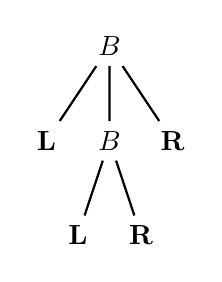
\begin{tikzpicture}[level distance=1.2cm, sibling distance=0.8cm, thick]
                            \node {$B$}
                                child {node {$\mathbf{L}$}}
                                child {node {$B$}
                                    child {node {$\mathbf{L}$}}
                                    child {node {$\mathbf{R}$}}
                                }
                                child {node {$\mathbf{R}$}};
                        \end{tikzpicture}
                        }
                        \vspace{0.2cm}\\
                        \footnotesize{
                        $0.\overline{1} \times 0.\overline{4} \approx 4.9\%$ \\
                        Likelihood
                        }
                    \end{center}
                \end{column}
                
                % Tree B
                \begin{column}{0.5\textwidth}
                    \begin{center}
                        \textbf{Correction B: \texttt{()()}}
                        \vspace{0.2cm}\\
                        \scalebox{0.75}{
                        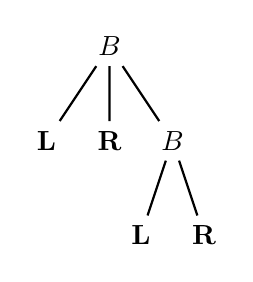
\begin{tikzpicture}[level distance=1.2cm, sibling distance=0.8cm, thick]
                            \node {$B$}
                                child {node {$\mathbf{L}$}}
                                child {node {$\mathbf{R}$}}
                                child {node {$B$}
                                    child {node {$\mathbf{L}$}}
                                    child {node {$\mathbf{R}$}}
                                };
                        \end{tikzpicture}
                        }
                        \vspace{0.2cm}\\
                        \footnotesize{
                        $0.\overline{3} \times 0.\overline{4} \approx 14.8\%$ \\
                        Likelihood
                        }
                    \end{center}
                \end{column}
            \end{columns}
        \end{column}
        
    \end{columns}

    \begin{center}
        \small{\textbf{Conclusion:} The algorithm prioritizes \texttt{(())} as a better correction for \texttt{))))}.}
    \end{center}
\end{frame}

\begin{frame}{Feature Attribution: The Ambiguity Problem}
    \begin{block}{Abductive Explanations (Errors)}
        $w = \texttt{))))}$ \\
        \vspace{0.1cm}
        \textcolor{blue}{\texttt{\underline{)}}}\texttt{)))},
        \texttt{)}\textcolor{blue}{\texttt{\underline{))}}}\texttt{)}
    \end{block}

    \vspace{0.4cm}
    
    % The transition block
    \begin{center}
    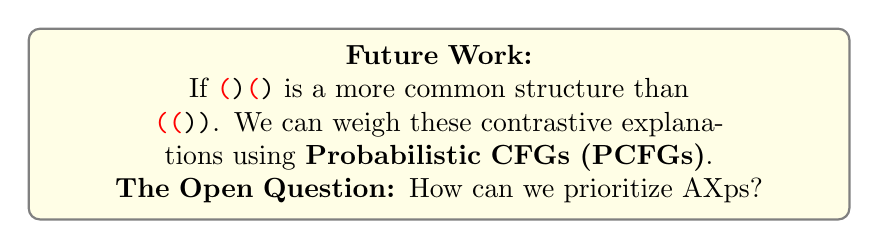
\begin{tikzpicture}[
        box/.style={rectangle, draw=black!50, fill=yellow!10, rounded corners, thick, text width=10cm, align=center, inner sep=6pt}
    ]
        \node[box] {
            \textbf{Future Work:}\\
            If \textcolor{red}{\texttt{(}}\texttt{)}\textcolor{red}{\texttt{(}}\texttt{)} is a more common structure than \textcolor{red}{\texttt{((}}\texttt{))}.
            We can weigh these contrastive explanations using \textbf{Probabilistic CFGs (PCFGs)}.
            
            \textbf{The Open Question:}
            How can we prioritize AXps?
        };
    \end{tikzpicture}
    \end{center}

\end{frame}

% \begin{frame}{Methodology: The CYK Algorithm}
%     \begin{itemize}
%         \item To verify if a word $w$ belongs to a Context-Free Language.
%     \end{itemize}
    
%     \vspace{0.2cm}

%     \begin{center}
%         \renewcommand{\arraystretch}{1.3}
%         \begin{tabular}{|c|c|c|c|}
%         \hline
%         \{L\} & \{B,P\} & $\emptyset$ & \textbf{\{B\}} \\ \cline{1-4}

%         \multicolumn{1}{c|}{$w_1=`('$} & \{R\} & $\emptyset$ & $\emptyset$ \\ \cline{2-4}

%         \multicolumn{1}{c}{} & \multicolumn{1}{c|}{$w_2=`)'$} & \{L\} & \{B,P\} \\ \cline{3-4}

%         \multicolumn{1}{c}{} & \multicolumn{1}{c}{} & \multicolumn{1}{c|}{$w_3=`('$} & $w_4=`)'$ \{R\} \\ \cline{4-4}

%         \multicolumn{1}{c}{} & \multicolumn{1}{c}{} & \multicolumn{1}{c}{} & \multicolumn{1}{c}{$w_4=`)'$} \\

%         \end{tabular}
%     \end{center}
%     \begin{center}
%         \renewcommand{\arraystretch}{1.3}
%         \begin{tabular}{|c|c|c|c|}
%         \hline
%         \{L\} & \{B,P\} & $\emptyset$ & \textbf{\{B\}} \\ \cline{1-4}

%         \multicolumn{1}{c|}{$w_1=`)'$} & \{R\} & $\emptyset$ & $\emptyset$ \\ \cline{2-4}

%         \multicolumn{1}{c}{} & \multicolumn{1}{c|}{$w_2=`)'$} & \{L\} & \{B,P\} \\ \cline{3-4}

%         \multicolumn{1}{c}{} & \multicolumn{1}{c}{} & \multicolumn{1}{c|}{$w_3=`)'$} & $w_4=`)'$ \{R\} \\ \cline{4-4}

%         \multicolumn{1}{c}{} & \multicolumn{1}{c}{} & \multicolumn{1}{c}{} & \multicolumn{1}{c}{$w_4=`)'$} \\

%         \end{tabular}
%     \end{center}
% \end{frame}


\begin{frame}{Methodology: The Modified CYK Algorithm}
    \begin{itemize}
        \item To verify if a set of indices $S$ is a valid CXp, we must check if replacing those tokens with wildcards ($\Sigma$) allows the word to be accepted.
        \item We achieve this by modifying the base case of the \textbf{CYK Parsing Algorithm}:
    \end{itemize}
    
    \vspace{0.2cm}
    \begin{block}{Modified Base Case Initialization}
        For each token $w_i$ at index $i$:
        \begin{itemize}
            \item \textbf{If $i \notin S$ (Fixed):} $T[i,i] = \{A \in V \mid A \to w_i\}$
            \item \textbf{If $i \in S$ (Freed/Wildcard):} $T[i,i] = \{A \in V \mid \exists \alpha \in \Sigma, A \to \alpha\}$
        \end{itemize}
    \end{block}
    
    \vspace{0.2cm}
    \small{\textit{Result: If the Start symbol $S$ appears at the top of the table $T[1,n]$, then the candidate set $S$ is a valid CXp.}}
\end{frame}



\begin{frame}{Visualizing Extraction: Greedy Deletion}
    \textbf{Algorithm Insight:} We start by freeing the \textit{entire} word, then greedily lock tokens back into place one by one. If locking a token breaks the parsing, it belongs in our minimal CXp.

    \vspace{0.3cm}
    \textbf{Example: $w = \texttt{))))}$, checking CXp candidate $S = \{1, 2\}$}
    
    % A simplified visual of the CYK bottom row to avoid overwhelming the slide
    \begin{center}
    \begin{tikzpicture}[
        cell/.style={rectangle, draw, minimum width=1.5cm, minimum height=0.8cm, align=center, font=\small},
        lbl/.style={font=\footnotesize\ttfamily}
    ]
        % Base row nodes
        \node[cell, fill=red!10] (c1) {\{L, R\}};
        \node[cell, fill=red!10, right=0cm of c1] (c2) {\{L, R\}};
        \node[cell, right=0cm of c2] (c3) {\{R\}};
        \node[cell, right=0cm of c3] (c4) {\{R\}};
        
        % Labels below
        \node[lbl, below=0.1cm of c1] {$w_1 = \Sigma$};
        \node[lbl, below=0.1cm of c2] {$w_2 = \Sigma$};
        \node[lbl, below=0.1cm of c3] {$w_3 = \texttt{)}$};
        \node[lbl, below=0.1cm of c4] {$w_4 = \texttt{)}$};
        
        % Annotation
        %\node[above=0.3cm of c1, font=\footnotesize\color{red!70!black}, xshift=0.75cm] {Freed indices act as wildcards};
        \node[above=0.3cm of c1, font=\footnotesize\color{red!70!black}, xshift=0.75cm] {Wildcards};
        \node[above=0.3cm of c3, font=\footnotesize\color{blue!70!black}, xshift=0.75cm] {Fixed indices lock to $R \to \texttt{)}$};
    \end{tikzpicture}
    \end{center}
    
    \vspace{0.1cm}
    \small{Because indices 1 and 2 can now act as \texttt{L} ($L \to \texttt{(}$), the CYK table successfully resolves to the Start variable, proving $\{1, 2\}$ is a valid explanation.}
\end{frame}

% --- SLIDE 5 ---
\begin{frame}{Current Status: CFG Explanations}
    \begin{itemize}
        \item \textbf{Theoretical Foundation:} 
        \begin{itemize}
            \item Formalized the extension of AXps/CXps to Context-Free Languages.
            \item Proved the correctness of the Modified CYK approach for wildcard evaluation.
        \end{itemize}
        \vspace{0.3cm}
        \item \textbf{Algorithmic Implementation:}
        \begin{itemize}
            \item Currently implementing the greedy extraction algorithm (\textsc{ExtractCXp}).
            \item Testing extraction performance on standard balanced parenthesis (Dyck) languages.
        \end{itemize}
        \vspace{0.3cm}
        \item \textbf{Next Immediate Step:} Benchmarking the computational complexity of the CYK-based extraction and drafting the manuscript for this second phase of the thesis.
    \end{itemize}
\end{frame}

